\section{Chapter 8 System Design and Algorithmic Framework}

\subsection{8.1 Introduction}

This chapter presents the detailed system design and algorithmic framework of the proposed CloudSentinel AI system. While the previous chapter introduced the overall architecture and research methodology, this chapter focuses on the internal design of each module, the interaction among components, and the algorithms responsible for cloud security analysis. The proposed framework follows a modular architecture in which each component performs a dedicated function while exchanging structured information with other modules. This modular approach improves maintainability, scalability, and extensibility, allowing future integration with additional cloud providers and security services.

\subsection{8.2 Overall System Design}

CloudSentinel AI consists of eight interconnected modules that collectively perform cloud security assessment. The major modules are:

\begin{enumerate}
\def\labelenumi{\arabic{enumi}.}
\tightlist
\item
  Cloud Asset Collector\\
\item
  Configuration Analyzer\\
\item
  Knowledge Graph Builder\\
\item
  Rule Engine\\
\item
  Attack Graph Generator\\
\item
  Context-Aware Risk Engine\\
\item
  Explainable AI Module\\
\item
  Dashboard and Reporting Module
\end{enumerate}

The interaction between these modules follows a sequential pipeline in which the output of one module serves as the input for the next. This design minimizes coupling between components while enabling independent testing and future enhancements.

\subsection{8.3 Module Design}

\subsubsection{8.3.1 Cloud Asset Collector}

\textbf{Purpose:} The Cloud Asset Collector is responsible for discovering cloud resources and collecting metadata from the cloud environment. It provides the raw information required for all subsequent stages of security analysis.\\
\textbf{Inputs:} AWS Access Key, Secret Key, Session Token, Region, AWS SDK (Boto3).\\
\textbf{Processing:} Authenticates with AWS APIs and retrieves metadata. Normalizes collected data into a common internal format.\\
\textbf{Outputs:} Cloud Asset Inventory, Configuration Metadata, Resource Dependency Information.

\subsubsection{8.3.2 Configuration Analyzer}

\textbf{Purpose:} The Configuration Analyzer evaluates cloud resources against predefined security policies and compliance standards.\\
\textbf{Inputs:} Cloud Asset Inventory, Configuration Metadata, Security Policies.\\
\textbf{Processing:} Evaluates resources against rules (e.g., Public S3, Open Security Group). Assigns initial severity levels.\\
\textbf{Outputs:} Misconfiguration Report, Initial Severity Scores.

\subsubsection{8.3.3 Knowledge Graph Builder}

\textbf{Purpose:} The Knowledge Graph Builder models the cloud environment as a graph.\\
\textbf{Inputs:} Cloud Resources, IAM Relationships, Network Relationships, Resource Ownership.\\
\textbf{Processing:} Represents cloud resources as nodes and relationships as edges (e.g., IAM Role \(\rightarrow\) EC2).\\
\textbf{Outputs:} Knowledge Graph, Resource Relationship Graph.

\subsubsection{8.3.4 Rule Engine}

\textbf{Purpose:} Evaluate security rules and compliance requirements.\\
\textbf{Inputs:} Knowledge Graph, Security Policies.\\
\textbf{Processing:} Evaluates resources against frameworks like CIS AWS Benchmark, AWS Best Practices, NIST, and Organization Policies.\\
\textbf{Outputs:} Rule Violations, Compliance Report.

\subsubsection{8.3.5 Attack Graph Generator}

\textbf{Purpose:} Identify realistic attack paths across the cloud infrastructure.\\
\textbf{Inputs:} Knowledge Graph, Rule Violations.\\
\textbf{Processing:} Traverses the graph to identify connected resources that may be exploited sequentially (e.g., Internet \(\rightarrow\) EC2 \(\rightarrow\) IAM Role \(\rightarrow\) Secrets Manager \(\rightarrow\) S3).\\
\textbf{Outputs:} Attack Graph, Attack Chains, Reachability Report.

\subsubsection{8.3.6 Context-Aware Risk Engine}

\textbf{Purpose:} Calculate contextual risk scores.\\
\textbf{Inputs:} Attack Graph, Asset Criticality, Business Context, Network Exposure, Identity Privileges.\\
\textbf{Processing:} Evaluates factors like attack complexity, sensitive data, and network exposure to generate dynamic risk scores.\\
\textbf{Outputs:} Dynamic Risk Score, Prioritized Findings.

\subsubsection{8.3.7 Explainable AI Module}

\textbf{Purpose:} Generate human-readable security explanations.\\
\textbf{Inputs:} Risk Scores, Attack Graph, Rule Violations.\\
\textbf{Processing:} LLM interprets technical findings and generates reports including security issues, causes, attack scenarios, and remediation.\\
\textbf{Outputs:} AI Report, Remediation Suggestions.

\subsubsection{8.3.8 Dashboard and Reporting Module}

\textbf{Purpose:} Present findings to analysts.\\
\textbf{Inputs:} Risk Scores, Attack Graph, AI Report.\\
\textbf{Processing:} Organizes information into interactive views, including inventory, risk dashboard, and visualization.\\
\textbf{Outputs:} Interactive Dashboard, PDF Report.

\subsection{8.4 Algorithmic Framework}

The proposed framework employs several algorithms:

\subsubsection{8.4.1 Algorithm 1 -- Cloud Asset Collection}

\textbf{Objective:} Collect metadata from AWS services.\\
\textbf{Time Complexity:} O(n) where n is the number of resources.

\subsubsection{8.4.2 Algorithm 2 -- Knowledge Graph Construction}

\textbf{Objective:} Transform cloud resources into a graph.\\
\textbf{Time Complexity:} O(V + E) where V is resources and E is relationships.

\subsubsection{8.4.3 Algorithm 2 -- Attack Path Generation}

\textbf{Objective:} Generate possible attack paths.\\
\textbf{Time Complexity:} O(V + E) for graph traversal.

\subsubsection{8.4.4 Algorithm 4 -- Context-Aware Risk Scoring}

\textbf{Objective:} Calculate contextual risk.\\
\textbf{Time Complexity:} O(n) where n is the number of attack paths.

\subsubsection{8.4.5 Algorithm 5 -- Explainable AI Generation}

\textbf{Objective:} Generate human-readable explanations.\\
\textbf{Note:} Execution time depends on LLM latency.

\subsection{8.5 Chapter Summary}

This chapter presented the detailed system design and algorithmic framework of CloudSentinel AI. Each module was described in terms of its purpose, inputs, processing logic, outputs, and advantages. Additionally, the core algorithms responsible for asset collection, knowledge graph construction, attack path generation, contextual risk scoring, and Explainable AI were introduced. The modular architecture and algorithmic framework provide a clear technical blueprint for implementing the proposed system.

\subsection{Additional Figures}

\begin{figure}
\hypertarget{fig:8_1}{%
\centering
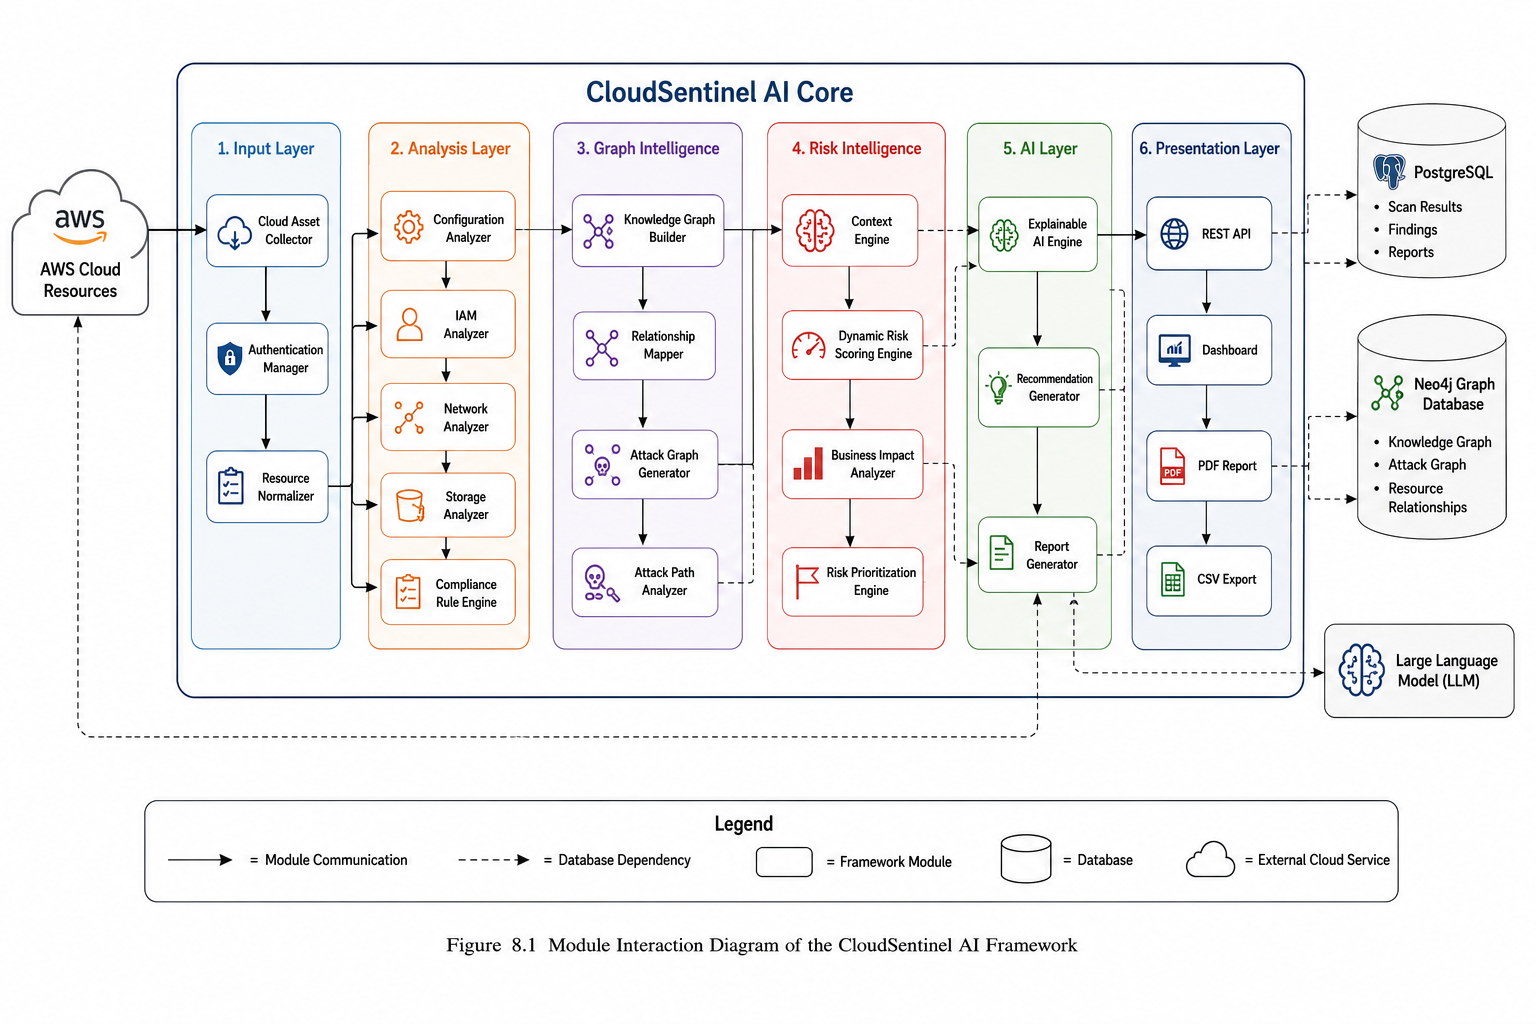
\includegraphics[width=0.9\textwidth,height=\textheight]{figures/image-8.1.png}
\caption{System Design and Algorithmic Framework.}\label{fig:8_1}
}
\end{figure}
